\chapter{Science Outside the Classroom}

\begin{multicols}{2}

\section{Science Clubs}

\begin{center}
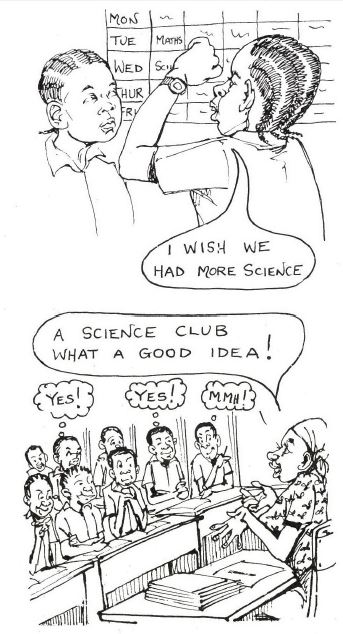
\includegraphics[width=0.45\textwidth]{./img/source/science-clubs.jpg}
\end{center}

A science club is an association of young
people, with one or more adult sponsors,
organised to carry out extra-curricular science
activities. The nature of this out-of-school
science education should be such that it both
complements and supplements science
education in school. 

It should include those
activities that are not easily provided at school,
and also those that the constraints of the
curriculum or time usually exclude. Out-of-school
science education can emphasize the
role of science in the community or encourage
creativity among young people and be a valuable
means of linking education with productive
work.


\subsection{Organizing a Club}

\begin{center}
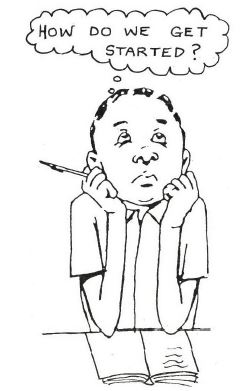
\includegraphics[width=0.25\textwidth]{./img/source/organizing-club.jpg}
\end{center}

The ideas for a new science or JETS (Junior
Engineers, Technologists and Scientists) club
may come from students or the teacher. Before
rushing into establishing the club the following
questions must be considered:

\begin{itemize}
\item Is it for science alone
or could it include other areas (engineering and
technology)?
\item Are they any other clubs/ Has
there been a science club in the past? If so, why
did it fail?
\item Are there any regulations (school or
elsewhere) which might affect the formation of
the club?
\item Does the constitution have to be
approved?
\item Where and when can the club meet?
\item Does the club need funds to operate? Where will
this money come from?
\item What do other staff
members think? Do others want to be involved?
\end{itemize}

The teacher or sponsor should call the first
meeting to establish the structure and scope of
the club. It is better to start off with a small club
with modest aims than to be over ambitious.
While the adult sponsor is vital to the success of
a club, she/he cannot and should not be expected
to do all the work. She/he should act as an
adviser helping when needed. Nevertheless
sponsors must be willing to give generously of
her/his time. A real interest and enthusiasm are
the keys to success! Enthusiasm is contagious,
but so is lack of enthusiasm!

\subsection{Activities Record Book}

\begin{center}
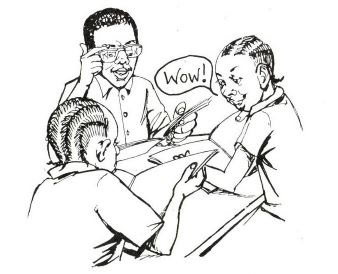
\includegraphics[width=0.45\textwidth]{./img/source/record-book-alt.jpg}
\end{center}

The club should keep a detailed record of the
science activities carried out at each meeting.
These should include judgments on the success
or failure of an activity. Many teachers keep
their own personal note book record of successful
activities, which they are able to add to
throughout their teaching career. Most of the
activities described in the \emph{Shika Express} companion manuals are ideal for use as out-of-
school activities.

\subsection{Science Notice Board}

\begin{center}
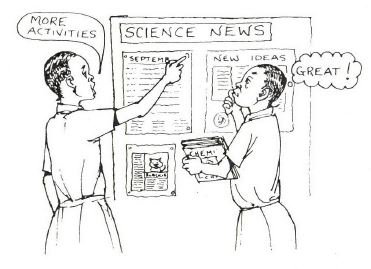
\includegraphics[width=0.49\textwidth]{./img/source/notice-board.jpg}
\end{center}

Display newspaper and magazine articles on
a science notice board. Notices giving dates and
times of regular meetings and special events can
be included. Why not hold a poster competition
to see who can create the most attractive or
imaginative work. Why not ask club members
to write essays on science topics for the board?

\subsection{Science in the News Book}

\begin{center}
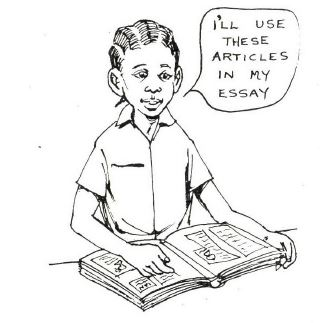
\includegraphics[width=0.45\textwidth]{./img/source/science-news.jpg}
\end{center}

Keep up with current scientific affairs and
general knowledge by keeping all selected
newspaper and magazine cuttings in a permanent
album. Build up a library of cuttings over your
school years.

Newspaper cuttings are an ideal source of
information for essays or quiz questions.

\subsection{Personal Science Kits}

\begin{center}
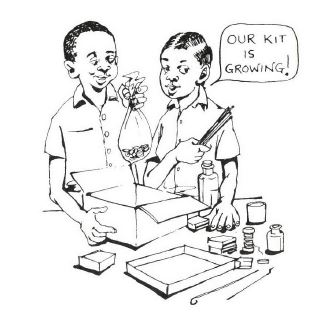
\includegraphics[width=0.45\textwidth]{./img/source/science-kits.jpg}
\end{center}

Students could start to collect items for their
own science kits. Why not hold a science kit
competition? Ask groups of students to collect
low or no cost materials from the local
environment which could be used for science
activities.

\subsection{Collections and Research}

\begin{center}
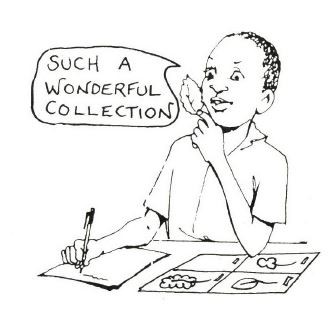
\includegraphics[width=0.45\textwidth]{./img/source/collections-research.jpg}
\end{center}

Students can make collections of a wide
variety of objects. Here are some ideas: rocks
and minerals; shells; types of wood; leaves;
flowers; bones; natural and artificial fabrics;
metals; stamps; types of paper and card.
Collections can be mounted labeled and
displayed in the science corner.

\subsection{Additional Practicals}

\begin{center}
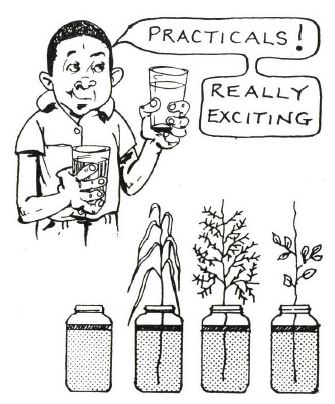
\includegraphics[width=0.45\textwidth]{./img/source/extra-practicals.jpg}
\end{center}

Students get the opportunity to do interesting
science practicals which may not be in their text
books or syllabus.


\section{Science Fairs}

\begin{center}
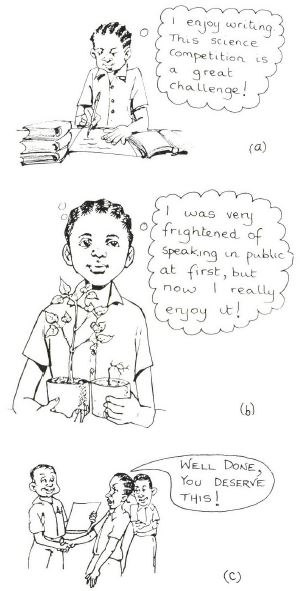
\includegraphics[width=0.45\textwidth]{./img/source/science-fairs.jpg}
\end{center}

Science fairs can be an excellent motivation
for science club activities. These could involve
exhibitions of projects, essay writing
competitions (a), project presentations (b),
debates (c), with certificates for prize winners.
Organisers should note that the presentation of
certificates, prizes or awards may increase the
basic running costs of the club. A sponsor from
local industry, business or community group
could be sought.

\section{Science Competitions}

Students love to compete and show their knowledge of math and science! Organize a small competition among interested students or create a multi-day competition using a variety of activities. See the \emph{Shika na Mikono} resource manuals for plenty of great competition activities.


\section{Science Conferences \hfill \\ and Camps}

\begin{center}
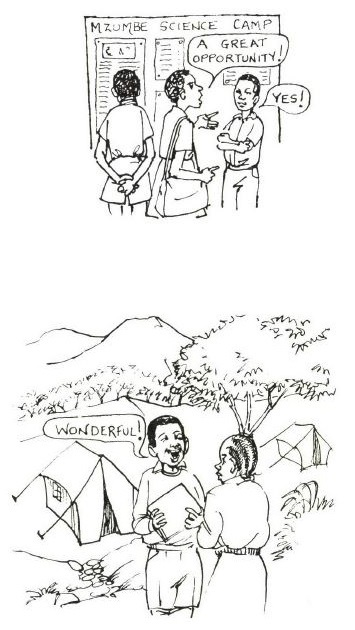
\includegraphics[width=0.49\textwidth]{./img/source/science-camps.jpg}
\end{center}

Science camps can be organised during the
holidays. These can be for a few days or several
weeks. As well as giving students the opportunity
to gain first hand knowledge it also gives
youngsters the chance to live and work together
with their peers and supportive adults.

There are two main types of camp:
\begin{enumerate}
\item[(a)] held in an
established institution like a school, college,
university, or special study centre.
\item[(b)] may
involve outdoor camping often in a remote
setting, to carry out a set research project.
\end{enumerate} 
If a camp is located at an institution the activities
may be more laboratory based and involve the
design, construction and testing of apparatus in
order to study specific topics. The nature of the
activities at an outdoor camp will depend on the
location chosen.

See the \emph{Shika na Mikono} resource manual for more information on holding math and science conferences and other events.


\section{Field Trips}

\begin{center}
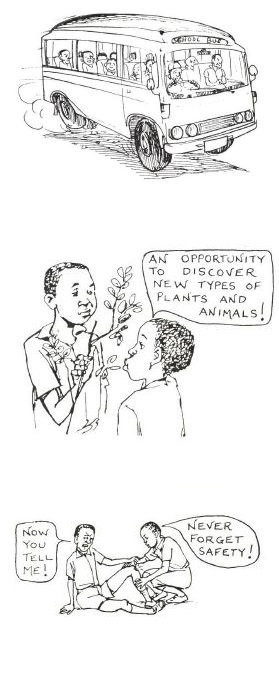
\includegraphics[width=0.45\textwidth]{./img/source/field-trips.jpg}
\end{center}

A scientific excursion may have a variety of
objectives, but it is very important that the major
objectives are known before the visit starts. If
possible an initial planning visit is made by the
teacher (or sponsor) to the excursion site, in
order to familiarise themselves with the local
environment and discover any difficulties.
Detailed forward planning is often the secret to
a successful visit. Meeting local resource persons
could lead to an altering of plans. Planning must
include the very important topics of finance and
safety!


\end{multicols}